\documentclass[11pt, oneside]{article}   	% use "amsart" instead of "article" for AMSLaTeX format
\usepackage{geometry}                		% See geometry.pdf to learn the layout options. There are lots.
\geometry{letterpaper}                   		% ... or a4paper or a5paper or ... 
%\geometry{landscape}                		% Activate for rotated page geometry
%\usepackage[parfill]{parskip}    		% Activate to begin paragraphs with an empty line rather than an indent
\usepackage{graphicx}				% Use pdf, png, jpg, or eps§ with pdflatex; use eps in DVI mode
								% TeX will automatically convert eps --> pdf in pdflatex		
\usepackage{amssymb}
\usepackage[utf8]{inputenc}
\usepackage[english]{babel}
\usepackage{amsmath} 
\usepackage{caption}
\usepackage{subcaption}
\usepackage{enumitem}
\newtheorem{theorem}{Theorem}
 
%SetFonts

%SetFonts


\title{Proof by Induction}
\author{Fahmida Hamid}
%\date{}							% Activate to display a given date or no date

\begin{document}
\maketitle
%\section{Proof 01}
\begin{theorem}
Show that every graph with two of more nodes contains two nodes that have equal degrees.
\end{theorem}
{\bf Basis:} A graph $G$ with two nodes must be one of the two followings:
\begin{figure}[ht]
\centering
\begin{subfigure}{.5\textwidth}
  \centering
  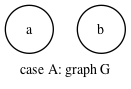
\includegraphics[width=.4\linewidth]{graphs}
  %\caption{A subfigure}
  %\label{fig:sub1}
\end{subfigure}%
\begin{subfigure}{.5\textwidth}
  \centering
  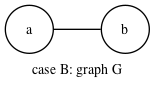
\includegraphics[width=.4\linewidth]{graphs1}
  %\caption{A subfigure}
  %\label{fig:sub2}
\end{subfigure}
%\caption{A figure with two subfigures}
\label{fig:test}
\end{figure}
In both cases, we see that $a$ and $b$ have the same degree. Therefore, the statement holds.\\
\par {\bf Inductive Hypothesis:} Let's assume that the statement holds for any graph $G = (V, E)$ with vertices $|V| = k\ge 2$.\\
\par {\bf Induction Step:} 
Let's assume, we have a graph $G' = (V', E')$ with $|V'| = k+1$ many vertices. If we assume that no two vertices share the same degree then the degree of any vertex $w \in V'$ will range from $0$ to $k$. \\

However not all the vertices with different degrees can occur in the same graph because a vertex with degree $0$ cannot co-exist with a vertex with degree $k$. So, there are vertices with degree $1$ to $k$. So, $G'$ can exhibit at most $k$ values among it's $k+1$ vertices. According to pigeon hole principle, there is at least two vertices that have equal degrees.\\
\iffalse
\par Now, we randomly select a vertex $w$ from $G'$; remove $w$ and it's incident edges from the graph. This way we construct a new graph $G'' = (V'', E'')$ with $|V| = k$. According to the inductive hypothesis, any graph with $k$ vertices contains two nodes with equal degrees. Let's assume, $u$ and $v$ are the two vertices in $G''$ with equal degrees. The vertex $w$ must satisfy one of the four following cases:
 
%Let's assume, we have a graph $G=(V, E)$ with $|V|= k$ vertices where two vertex $u$ and $v$ have equal degree. Now, let's add a new vertex $w$ to $G$ and form a new graph $G'$ with $k+1$ vertices. We need to consider the following cases:\\
\hspace{10 pt}
\begin{description}[noitemsep, nolistsep]
\item [Case 0: ] The degree of $w$ is zero. 
\item [Case 1: ] $w$ is connected to both $u$ and $v$.
\item [Case 2: ] $w$ is connected to some vertices in $V \setminus \{u,v\}$.
\item [Case 3: ] $w$ is connected to $u$ and some vertices in $ V \setminus v$. The alternate possible option will have the same impact over the statement. 
\end{description}
\hspace{10 pt}
Now, the degree of any node $w$ in $G'$ cannot be zero.

%\par For case 0, 1, and 2, the degree of $u$ and $v$ in $G'$ remains equal. Thus the statement follows for a graph $G'$ with $k+1$ vertices if it is true for a graph $G''$ with $k$ vertices.\\
%\par Certainly for case 3, the degree of $u$ and $v$ is not equal in $G'$ though they are equal in $G''$ (a sample from figure \ref{fig:test}).  We need to carefully consider that the two vertices with equal degrees in $G''$ do not have to have equal degrees in $G'$. To avoid falling into case 3, we can pick the vertex (that we want to delete) in such a way that it has no neighbors or at least two neighbors. That way, we can guarantee to find one vertex that satisfies either case 0, 1, or 2.


\begin{figure}[ht]
\centering
\begin{subfigure}{.5\textwidth}
  \centering
  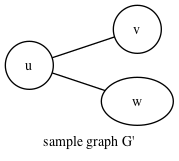
\includegraphics[width=.4\linewidth]{graphs2}
  %\caption{A subfigure}
  %\label{fig:sub1}
\end{subfigure}%
\begin{subfigure}{.5\textwidth}
  \centering
  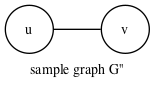
\includegraphics[width=.4\linewidth]{graphs3}
  %\caption{A subfigure}
  %\label{fig:sub2}
\end{subfigure}
\caption{Constructing $G''$ from $G'$}
\label{fig:test}
\end{figure}


%Let's delete $v$ and it's associated edges from $G'$. Now we have a new graph $G'' = (V'', E'')$ with $V'' = V \setminus v \cup \{w\} $ vertices. Note that $|V''| = k$ as we have removed one vertex $v$ from $G$ and added one $w$.\\
%According to the inductive hypothesis, any graph (like $G$ or $G''$) with $k$ vertices have two nodes with equal degree. So there must be two vertices in $G''$ with equal degree. Therefore, in $G'$ (after including $w$ to $G$), if the degree of $u$ and $v$ becomes unequal, there will be other two possible vertices with equal degrees.\\
\fi
\par Hence, every graph with two of more nodes contains two nodes that have equal degrees.
%\subsection{}



\end{document}  